%-----------------------------------------------------------------------------%
% \listoftables
\chapter{\babTiga}


%-----------------------------------------------------------------------------%
% \lipsum[6-6]

%-----------------------------------------------------------------------------%
\section{Kedudukan dan Koordinasi}
%-----------------------------------------------------------------------------%

Selama pelaksanaan kerja magang di PT Ganda Visi Jayatama, penulis tergabung dalam tim pengembangan sistem CHRIS (Concise Human Resources Information System), dan berperan sebagai Backend Engineer Intern. Dalam peran ini, penulis bertanggung jawab dalam proses pengembangan dan pengujian Application Programming Interface (API) yang digunakan oleh sistem, serta melakukan kolaborasi dengan anggota tim lainnya dalam menyusun dan menyempurnakan fitur-fitur sistem kepegawaian berbasis web.

Tim CHRIS terdiri dari beberapa anggota dengan peran yang saling terintegrasi. Bimbingan diberikan oleh Bapak Edo Setiawan selaku Supervisor sekaligus Head of Development, yang secara rutin melakukan evaluasi mingguan terhadap progres serta melakukan \textit{code review} terhadap hasil pengembangan backend. Koordinasi teknis lebih lanjut juga dilakukan bersama Bapak Muhammad Alwin Alamsyah Handoko Putra selaku Backend Lead, yang memimpin diskusi internal tim backend setiap hari Jumat dalam Backend Internal Meeting. Perencanaan dan distribusi tugas dikoordinasikan oleh Project Manager, Ibu Keshia Tiffany, yang bertanggung jawab membagi \textit{backlog} tugas kepada anggota tim, serta melakukan sesi evaluasi pribadi (\textit{one-on-one}) dengan masing-masing anggota tim magang. Dalam pengembangan tampilan antarmuka sistem, penulis berkolaborasi dengan Designer Amanda Citra Dewanti yang membuat wireframe dan desain hi-fi, serta dua Frontend Engineer Intern, Amanda Citra Dewanti dan Calista Belva, yang bertugas membangun tampilan web menggunakan React. Sementara itu, penulis dan rekan satu tim, Kevin Ken, menjalankan peran sebagai Backend Engineer menggunakan Express.js dan Node.js untuk pengembangan API, serta PostgreSQL sebagai sistem basis data.

Seluruh kegiatan kerja magang dilakukan secara langsung di kantor (Work From Office). Koordinasi dilakukan melalui daily standup setiap pagi untuk melaporkan progres harian, menyampaikan rencana kerja, serta mendiskusikan kendala yang dihadapi. Setiap dua minggu sekali, tim juga melaksanakan sprint retrospective untuk mengevaluasi hasil kerja dalam satu sprint dan menentukan perbaikan serta target sprint berikutnya. Penugasan proyek dikelola menggunakan platform Jira (Atlassian) dalam bentuk backlog sprint yang dibagikan kepada setiap anggota tim secara terstruktur dan terukur.


% \noindent \begin{align}\label{eq:garis}
% 	\cfrac{y - y_{1}}{y_{2} - y_{1}} = 
% 	\cfrac{x - x_{1}}{x_{2} - x_{1}}
% \end{align}

% \equ~\ref{eq:garis} di atas adalah persamaan garis. 
% \equ~\ref{eq:garis} dan \ref{eq:bola} sama-sama dibuat dengan perintah \bslash
% align. 
% Perintah ini juga dapat digunakan untuk menulis lebih dari satu persamaan. 

% \noindent \begin{align}\label{eq:bola}
% 	\underbrace{|\overline{ab}|}_{\text{pada bola $|\overline{ab}| = r$}} 
% 		= \sqrt[2]{(x_{b} - x_{a})^{2} + (y_{b} - y_{a})^{2} + 
% 				\vert\vert(z_{b} - z_{a})^{2}}
% \end{align}

%-----------------------------------------------------------------------------%
\section{Tugas yang Dilakukan}
\label{sec:multiEqu}
%-----------------------------------------------------------------------------%

Selama pelaksanaan kerja magang di PT Ganda Visi Jayatama, penulis diberikan tanggung jawab utama dalam satu proyek utama, yaitu pengembangan aplikasi \textit{Internal System}. Tugas-tugas yang dijalankan selama magang terbagi ke dalam beberapa aktivitas utama sebagai berikut:

\begin{enumerate}
    \item Mengembangkan API untuk kebutuhan aplikasi \textit{Internal System}, yang mencakup pembuatan fitur-fitur backend sesuai dengan spesifikasi fungsional.
    \item Melakukan dokumentasi terhadap API yang telah dikembangkan menggunakan platform dokumentasi API, Apidog.
    \item Melakukan pengujian secara mandiri terhadap API yang dibuat untuk memastikan bahwa seluruh endpoint berjalan sesuai dengan fungsinya, serta menangani error handling dan validasi data.
\end{enumerate}


% %-----------------------------------------------------------------------------%
% \section{Membuat Tabel}
% %-----------------------------------------------------------------------------%
% Seperti pada gambar, tabel juga dapat diberi label dan caption. 
% Caption pada tabel terletak pada bagian atas tabel. 
% Contoh tabel sederhana dapat dilihat pada \tab~\ref{tab:tab1}.

% \begin{table}
% 	\centering
% 	\caption{Contoh Tabel}
% 	\label{tab:tab1}
% 	\begin{tabular}{l | c r}
% 		\hline
% 		& kol 1 & kol 2 \\ 
% 		\hline
% 		baris 1 & 1 & 2 \\
% 		baris 2 & 3 & 4 \\
% 		baris 3 & 5 & 6 \\
% 		jumlah  & 9 & 12 \\
% 		\hline
% 	\end{tabular}
% \end{table}

% Ada jenis tabel lain yang dapat dibuat dengan \latex~berikut 
% beberapa di antaranya. 
% Contoh-contoh ini bersumber dari 
% \url{http://en.wikibooks.org/wiki/LaTeX/Tables}

% \begin{table}
% 	\centering
% 	\caption{An example of rows spanning multiple columns}
% 	\label{row.spanning}
% 	\begin{tabular}{l l *{6}{c}}
%   		\hline % create horizontal line
%   		No & Name & \multicolumn{3}{c}{Week 1} & \multicolumn{3}{c}{Week 2} \\
%   		\cline{3-8} % create line from 3rd column till 8th column
%   		& & A & B & C & A & B & C\\
%   		\hline
%   		1 & Lala & 1 & 2 & 3 & 4 & 5 & 6\\
%   		2 & Lili & 1 & 2 & 3 & 4 & 5 & 6\\
%   		3 & Lulu & 1 & 2 & 3 & 4 & 5 & 6\\
%   		\hline
% 	\end{tabular}
% \end{table}

% \lipsum[43-44]

% \begin{table}
% 	\centering
% 	\caption{Penulisan judul tabel dan judul gambar adalah rata kiri kanan serta tidak dicetak tebal dan mengikuti cara penulisan kalimat (sentence case).}
% 	\label{column.spanning}
% 	\begin{tabular}{l c l}
% 		\hline
% 		Percobaan & Iterasi & Waktu \\
% 		\hline
% 		Pertama & 1 & 0.1 sec \\ \hline
% 		\multirow{2}{*}{Kedua} & 1 & 0.1 sec \\
%  		& 3 & 0.15 sec \\ 
%  		\hline
% 		\multirow{3}{*}{Ketiga} & 1 & 0.09 sec \\
%  		& 2 & 0.16 sec \\
%  		& 3 & 0.21 sec \\ 
%  		\hline
% 	\end{tabular}\\
% 	\vspace{1em}
% 	{\small Sumber: \url{http://en.wikibooks.org/wiki/LaTeX/Tables}}
% \end{table}


% \lipsum[45-46]

% \noindent \begin{align}\label{eq:matriks}	
% 	|\overline{a} * \overline{b}| &= |\overline{a}| |\overline{b}| \sin\theta 
% 		\\[0.2cm]
% 	\overline{a} * \overline{b} &=  
% 		\begin{array}{| c c c |}
% 			\hat{i} & x_{1} & x_{2} \\
% 			\hat{j} & y_{1} & y_{2} \\
% 			\hat{k} & z_{1} & z_{2} \\
% 		\end{array} \nonumber \\[0.2cm]
% 	&= \hat{i} \,
% 		\begin{array}{ | c c | }
% 			y_{1} & y_{2} \\
% 			z_{1} & z_{2} \\
% 		\end{array} 
% 	   + \hat{j} \,
% 		\begin{array}{ | c c | }
% 			z_{1} & z_{2} \\
% 			x_{1} & x_{2} \\
% 		\end{array} 
% 	   + \hat{k} \,	
% 		\begin{array}{ | c c | }
% 			x_{1} & x_{2} \\
% 			y_{1} & y_{2} \\
% 		\end{array}
% 		\nonumber
% \end{align}

% Pada \equ~\ref{eq:matriks} dapat dilihat beberapa baris menjadi satu bagian 
% dari \equ~\ref{eq:matriks}. 
% Sedangkan di bawah ini dapat dilihat bahwa dengan cara yang sama, \equ~
% \ref{eq:gabungan1}, \ref{eq:gabungan2}, dan \ref{eq:gabungan3} memiliki nomor 
% persamaannya masing-masing. 

% \noindent \begin{align}\label{eq:gabungan1}	
% 	\int_{a}^{b} f(x)\, dx + \int_{b}^{c} f(x) \, dx = \int_{a}^{c} f(x) \, dx
% 		\\\label{eq:gabungan2}
% 	\lim_{x \to \infty} \frac{f(x)}{g(x)} = 0 \hspace{1cm} 
% 		\text{jika pangkat $f(x)$ $<$ pangkat $g(x)$} \\\label{eq:gabungan3}
% 	a^{m^{a \, ^{n}\log b }} = b^{\frac{m}{n}}
% \end{align}



% Rumus \ref{eq:Precision} menunjukkan cara perhintungan \textit{Precision}.

% \addequation{\textit{Precision}}{%
% \begin{equation}  \label{eq:Precision}
%     Precision = \frac{TP}{TP+FP}
% \end{equation}
% }

% Rumus \ref{eq:Recall} menunjukkan cara perhitungan \textit{Recall}.

% \addequation{\textit{Recall}}{
% \begin{equation}  \label{eq:Recall}
%     Recall = \frac{TP}{TP+FN}
% \end{equation}

% }

% \addequation{\textit{F1 Score}}{%
% \begin{equation}  \label{eq:F1-score}
%     F1 Score = 2*\frac{Precision*Recall}{Precision+Recall}
% \end{equation}
% }

% -----------------------------------------------------------------------------%
\section{Uraian Pelaksanaan Magang}
% -----------------------------------------------------------------------------%
Pelaksanaan kerja magang diuraikan seperti pada Tabel~\ref{tab:tbl_uraian}.

\begin{center}
\begin{longtable}{|c|p{0.75\textwidth}|}
\caption{Pekerjaan yang dilakukan tiap minggu selama pelaksanaan kerja magang}
\label{tab:tbl_uraian} \\
\hline
\textbf{Minggu Ke -} & \textbf{Pekerjaan yang dilakukan} \\
\hline
\endfirsthead

\multicolumn{2}{c}%
{{\tablename\ \thetable{} -- Pekerjaan yang dilakukan tiap minggu selama pelaksanaan kerja magang}} \\
\hline
\textbf{Minggu Ke -} & \textbf{Pekerjaan yang dilakukan} \\
\hline
\endhead

\hline \multicolumn{2}{|r|}{{Lanjut pada halaman berikutnya}} \\
\hline
\endfoot

\hline \hline
\endlastfoot

1 & Mempelajari boilerplate backend dan mulai mengembangkan API untuk Employee Status pada sistem CHRIS. \\
\hline
2 & Melanjutkan pengembangan dan penyempurnaan API Employee Status serta melakukan validasi ulang pada form Employee di sistem CHRIS. \\
\hline
3 & Melakukan revisi minor pada API employee form, menyelesaikan tabel User dan Employee Status, serta berpartisipasi dalam Sprint Retro. \\
\hline
4 & Mengembangkan fitur pagination untuk berbagai modul (User, Leave, Attendance), membuat API form pengajuan cuti, serta melakukan code review dan diskusi dalam monthly meeting. \\
\hline
5 & Fokus pada revisi dan pengembangan API perizinan cuti, integrasi dengan frontend, serta showcase sistem CHRIS dan implementasi pagination untuk Leave Types. \\
\hline
6 & Melakukan revisi dan filtering pada Leave Permit Dashboard, menambahkan fitur cancel, serta aktif dalam code review dan weekly meeting tim backend. \\
\hline
7 & Melakukan berbagai pengujian dan UAT untuk Leave Management, membangun sistem tree berbasis jabatan untuk izin, serta menangani revisi migrasi dan API CHRISM (CHRIS Mobile). \\
\hline
8 & Mengembangkan sistem hierarki supervisi berbasis tree, menerapkan biometrik pada login API, dan mulai membangun user report summary API serta mempersiapkan People Report. \\
\hline
9 & Fokus pada penyempurnaan fitur User Report, termasuk penambahan filter tanggal dan perbaikan minor, serta melakukan hashing biometrik dan refactor pada dashboard Leave Permit. \\
\hline
10 &  Memulai riset intensif terkait sistem Payroll dan skema tabelnya, membuat dokumentasi di Apidog.\\
\hline
11 &  Melanjutkan pengembangan API Payroll berdasarkan hasil riset skema tabel, memperbarui dokumentasi di Apidog, serta mengikuti kegiatan Backlog Planning dan Sprint Closing.\\
\hline
12 &  Fokus pada pengembangan lanjutan API Payroll termasuk fitur Create, Get, Update, dan Delete, serta mulai menangani logika data untuk User Allowances.\\
\hline
13 &  Melanjutkan secara intensif pengembangan API Payroll khusus untuk pengelolaan dan perhitungan Each User Allowances secara berkelanjutan sepanjang minggu.\\
\hline
14 &  Mulai mengembangkan dan menyempurnakan Salary Slip APIs serta melakukan bugfix dan refactor pada User Allowance dan konfigurasi Payroll untuk integrasi dengan frontend.\\
\hline
15 &  Menambahkan fitur penghapusan User Allowance, memperbaiki konfigurasi endpoint Payroll, dan membuat API gabungan untuk manajemen detail user, payroll, serta tunjangan.\\
\hline
16 &  Melanjutkan integrasi Salary Slip dengan frontend serta melakukan pengujian menyeluruh terhadap modul Payroll, Allowance, dan Salary Slip.\\
\hline
17 &  Melakukan perbaikan pada logika dan pagination Salary Slip serta Payroll Config, merevisi sistem, dan menyiapkan internal report serta showcase Payroll.\\
\hline

\end{longtable}
\end{center}

% \begin{table}
% 	\centering
% 	\caption{ Pekerjaan yang dilakukan tiap minggu selama pelaksanaan kerja magang}
% 	\label{tbl_uraian}
% 	\begin{tabular}{|c | p{0.75\textwidth}| }
% 		\hline
% 		Minggu Ke - & Pekerjaan yang dilakukan \\
% 		\hline
% 		1 & 
% 		Mempelajari boilerplate backend dan mulai mengembangkan API untuk Employee Status pada sistem CHRIS.\\
% 		\hline
%  		2 & 
% 		Melanjutkan pengembangan dan penyempurnaan API Employee Status serta melakukan validasi ulang pada form Employee di sistem CHRIS.\\
% 		\hline
%  		3 & 
% 		Melakukan revisi minor pada API employee form, menyelesaikan tabel User dan Employee Status, serta berpartisipasi dalam Sprint Retro. \\
%  		\hline
%  		4 & 
% 		Mengembangkan fitur pagination untuk berbagai modul (User, Leave, Attendance), membuat API form pengajuan cuti, serta melakukan code review dan diskusi dalam monthly meeting \\
%  		\hline
%  		5 & 
% 		Fokus pada revisi dan pengembangan API perizinan cuti, integrasi dengan frontend, serta showcase sistem CHRIS dan implementasi pagination untuk Leave Types.\\
%  		\hline
%  		6 & 
% 		Melakukan revisi dan filtering pada Leave Permit Dashboard, menambahkan fitur cancel, serta aktif dalam code review dan weekly meeting tim backend.\\
%  		\hline
%  		7 & 
% 		Melakukan berbagai pengujian dan UAT untuk Leave Management, membangun sistem tree berbasis jabatan untuk izin, serta menangani revisi migrasi dan API CHRISM (CHRIS Mobile).\\
%  		\hline
%  		8 & Mengembangkan sistem hierarki supervisi berbasis tree, menerapkan biometrik pada login API, dan mulai membangun user report summary API serta mempersiapkan People Report.\\
%  		\hline
%  		9 & \\
%  		\hline
%  		10 & \\
%  		\hline
% 	\end{tabular}
% \end{table}



%-----------------------------------------------------------------------------%
\section{Pengumpulan dan Analisis Kebutuhan}
%-----------------------------------------------------------------------------%
Kebutuhan sistem dalam proyek ini diperoleh melalui koordinasi langsung dengan supervisor dan tim backend internal. Sebagian besar requirement ditentukan secara iteratif berdasarkan kebutuhan bisnis dan sprint mingguan yang telah direncanakan oleh tim. Proses pengumpulan requirement dilakukan melalui diskusi teknis, retrospective meeting, dan task assignment harian.

Berikut ini adalah uraian requirement utama yang berhasil diidentifikasi dan diimplementasikan dalam proyek selama masa kerja praktik.

%-----------------------------------------------------------------------------%
\subsection{Kebutuhan}
%-----------------------------------------------------------------------------%
\subsubsection{Refaktor User Management dan Validasi Data}

Pengembangan dimulai dengan perbaikan sistem \textbf{User Management}, termasuk validasi \textit{form input} dan \textit{refactor} struktur tabel seperti \textbf{user} dan \textbf{employment status}. Hal ini bertujuan untuk memastikan integritas data pengguna dan kemudahan pengelolaan melalui backend maupun frontend.
%-----------------------------------------------------------------------------%
\subsubsection{Optimalisasi Leave Permit}

Modul \textbf{Leave Permit} dikembangkan agar lebih efisien dan intuitif. Perubahan meliputi \textit{refactor} pada proses \textit{form submission}, penambahan tombol pembatalan (\textit{cancel}) pengajuan cuti, serta tampilan daftar cuti untuk atasan. Fitur-fitur ini dirancang agar mencerminkan alur persetujuan yang realistis dan terstruktur.
%-----------------------------------------------------------------------------%
\subsubsection{Implementasi Pagination}

Untuk mendukung jumlah data yang besar, sistem pagination ditambahkan pada beberapa modul utama seperti User, Leave, dan Attendance. Hal ini dilakukan guna menjaga performa dan kenyamanan pengguna.
%-----------------------------------------------------------------------------%
\subsubsection{Pengembangan Sistem Hierarki}

Dibuat fungsi \textit{tree hierarchy} berdasarkan struktur jabatan untuk mendukung fitur-fitur seperti izin cuti (\textit{accept}/\textit{reject}) dan tampilan dashboard atasan. Fungsi ini menjadi dasar logika akses dan pengelolaan hubungan antar pegawai.
%-----------------------------------------------------------------------------%
\subsubsection{Modul Payroll dan Slip Gaji}

Modul \textbf{Payroll} dikembangkan untuk menghasilkan slip gaji yang dihitung berdasarkan tunjangan. Termasuk di dalamnya pengembangan API untuk CRUD data payroll, penyusunan salary slip, dan integrasi dengan frontend.
%-----------------------------------------------------------------------------%


%-----------------------------------------------------------------------------%
\subsection{Framework dan Aplikasi yang Digunakan}
%-----------------------------------------------------------------------------%

%-----------------------------------------------------------------------------%
\subsubsection{Express JS}

Framework backend berbasis Node.js yang digunakan untuk membangun REST API\@. Express dipilih karena ringan, fleksibel, dan cocok untuk kebutuhan proyek berbasis modul seperti CHRIS\@.
%-----------------------------------------------------------------------------%
\subsubsection{DBeaver}

DBeaver digunakan untuk pengelolaan database PostgreSQL secara visual. Tool ini memudahkan debugging query, analisis relasi, dan validasi data secara langsung.
%-----------------------------------------------------------------------------%
\subsubsection{Apidog}
Apidog dimanfaatkan sebagai platform dokumentasi dan testing API\@. \textit{Tool} ini membantu frontend untuk memahami struktur \textit{request}/\textit{response} dan berperan sebagai \textit{single source of truth} untuk komunikasi antar tim.
% ---------------------------------------------------------------------------------%
\clearpage
% ---------------------------------------------------------------------------------%
\section{Design System}
Bagian ini menjelaskan perancangan sistem yang mencakup struktur basis data dan alur sistem untuk fitur-fitur yang dikembangkan selama masa kerja praktik.

\subsection{Database Diagram}
Struktur basis data pada sistem CHRIS dirancang untuk mendukung modularitas fitur seperti User Management, Leave Permit, dan Payroll. 
Beberapa tabel baru ditambahkan serta dilakukan refaktor pada tabel eksisting guna meningkatkan efisiensi dan skalabilitas.

Adapun tabel yang dirancang atau dimodifikasi selama masa kerja praktik adalah sebagai berikut:

\begin{itemize}
    \item \textbf{users}: Menyimpan informasi dasar pegawai.
    \item \textbf{employment\_statuses}: Menyimpan status kepegawaian (misal: fulltime, intern).
    \item \textbf{permit\_records}: Menyimpan data pengajuan cuti oleh pegawai.
    \item \textbf{payroll\_configurations}: Menyimpan data jenis payroll yang akan digunakan yang sudah menyimpan preset allowances yang sudah terikat dengan payroll ini (dengan tujuan supaya HR tidak perlu mengisi allowance yang sudah ada dari Payroll Configuration ini).
    \item \textbf{allowance\_types}: Menyimpan data tunjangan yang ada pada sistem.
    \item \textbf{user\_allowances}: Menyimpan data jumlah tunjangan per pengguna yang digunakan dalam perhitungan gaji.
    \item \textbf{user\_payroll\_applications}: Menyimpan data pengguna dengan data payroll yang sudah pernah aktif.
\end{itemize}

\noindent Dokumentasi struktur tabel secara visual dapat dilihat pada Gambar \ref{fig:db-schema}.

\begin{figure}[H]
    \centering
    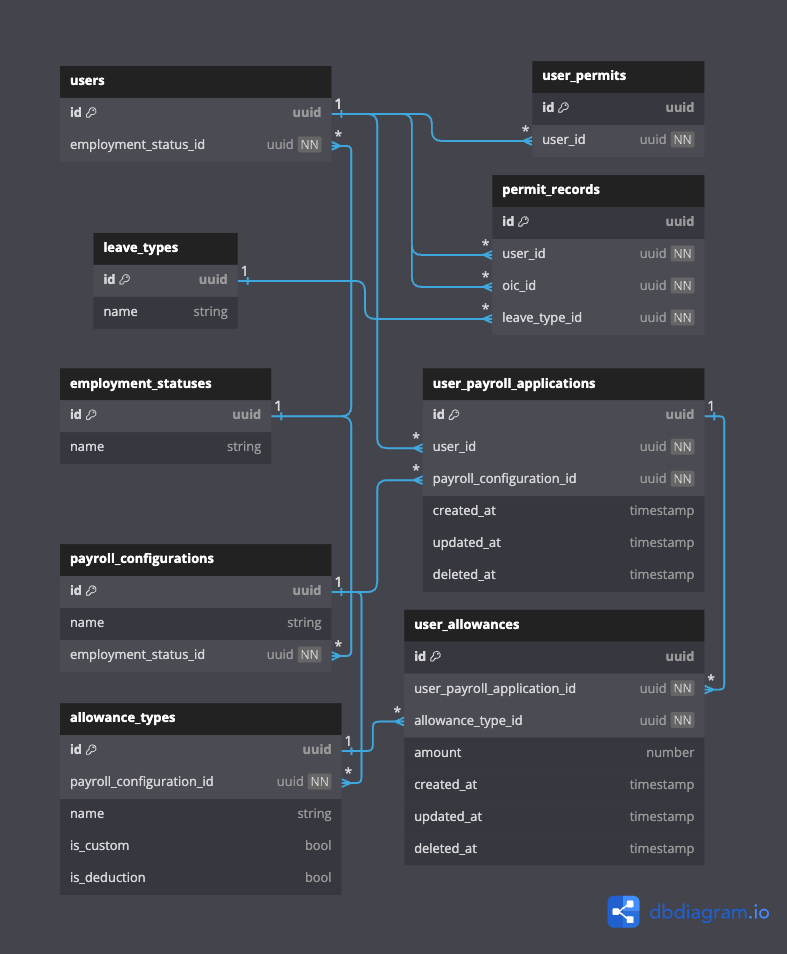
\includegraphics[width=1\textwidth]{assets/pics/fig_database_diagram.png}
    \caption{Database Diagram}
    \label{fig:db-schema}
\end{figure}



\subsubsection{Subsub-section}

\lipsum[13-14]


\begin{center}
\begin{longtable}{|l|l|l|}
\caption{A sample long table} \label{tab:long} \\

\hline \multicolumn{1}{|c|}{\textbf{First column}} & \multicolumn{1}{c|}{\textbf{Second column}} & \multicolumn{1}{c|}{\textbf{Third column}} \\ \hline 
\endfirsthead

\multicolumn{3}{c}%
{{ \tablename\ \thetable{} \small A sample long table (lanjutan)}} \\
\hline \multicolumn{1}{|c|}{\textbf{First column}} & \multicolumn{1}{c|}{\textbf{Second column}} & \multicolumn{1}{c|}{\textbf{Third column}} \\ \hline 
\endhead

\hline \multicolumn{3}{|r|}{{Lanjut pada halaman berikutnya}} \\ \hline
\endfoot

\hline \hline
\endlastfoot

One & abcdef ghjijklmn & 123.456778 \\
One & abcdef ghjijklmn & 123.456778 \\
One & abcdef ghjijklmn & 123.456778 \\
One & abcdef ghjijklmn & 123.456778 \\
One & abcdef ghjijklmn & 123.456778 \\
One & abcdef ghjijklmn & 123.456778 \\
One & abcdef ghjijklmn & 123.456778 \\
One & abcdef ghjijklmn & 123.456778 \\
One & abcdef ghjijklmn & 123.456778 \\
One & abcdef ghjijklmn & 123.456778 \\
One & abcdef ghjijklmn & 123.456778 \\
One & abcdef ghjijklmn & 123.456778 \\
One & abcdef ghjijklmn & 123.456778 \\
One & abcdef ghjijklmn & 123.456778 \\
One & abcdef ghjijklmn & 123.456778 \\
One & abcdef ghjijklmn & 123.456778 \\
One & abcdef ghjijklmn & 123.456778 \\
One & abcdef ghjijklmn & 123.456778 \\
One & abcdef ghjijklmn & 123.456778 \\
One & abcdef ghjijklmn & 123.456778 \\
One & abcdef ghjijklmn & 123.456778 \\
One & abcdef ghjijklmn & 123.456778 \\
One & abcdef ghjijklmn & 123.456778 \\
One & abcdef ghjijklmn & 123.456778 \\
One & abcdef ghjijklmn & 123.456778 \\
One & abcdef ghjijklmn & 123.456778 \\
One & abcdef ghjijklmn & 123.456778 \\
One & abcdef ghjijklmn & 123.456778 \\
One & abcdef ghjijklmn & 123.456778 \\
One & abcdef ghjijklmn & 123.456778 \\
One & abcdef ghjijklmn & 123.456778 \\
One & abcdef ghjijklmn & 123.456778 \\
One & abcdef ghjijklmn & 123.456778 \\
One & abcdef ghjijklmn & 123.456778 \\
One & abcdef ghjijklmn & 123.456778 \\
One & abcdef ghjijklmn & 123.456778 \\
One & abcdef ghjijklmn & 123.456778 \\
One & abcdef ghjijklmn & 123.456778 \\
One & abcdef ghjijklmn & 123.456778 \\
One & abcdef ghjijklmn & 123.456778 \\
One & abcdef ghjijklmn & 123.456778 \\
One & abcdef ghjijklmn & 123.456778 \\
One & abcdef ghjijklmn & 123.456778 \\
One & abcdef ghjijklmn & 123.456778 \\
One & abcdef ghjijklmn & 123.456778 \\
One & abcdef ghjijklmn & 123.456778 \\
One & abcdef ghjijklmn & 123.456778 \\
One & abcdef ghjijklmn & 123.456778 \\
One & abcdef ghjijklmn & 123.456778 \\
One & abcdef ghjijklmn & 123.456778 \\
One & abcdef ghjijklmn & 123.456778 \\
One & abcdef ghjijklmn & 123.456778 \\
One & abcdef ghjijklmn & 123.456778 \\
One & abcdef ghjijklmn & 123.456778 \\
One & abcdef ghjijklmn & 123.456778 \\
One & abcdef ghjijklmn & 123.456778 \\
One & abcdef ghjijklmn & 123.456778 \\
One & abcdef ghjijklmn & 123.456778 \\
One & abcdef ghjijklmn & 123.456778 \\
One & abcdef ghjijklmn & 123.456778 \\
One & abcdef ghjijklmn & 123.456778 \\
One & abcdef ghjijklmn & 123.456778 \\
One & abcdef ghjijklmn & 123.456778 \\
One & abcdef ghjijklmn & 123.456778 \\
One & abcdef ghjijklmn & 123.456778 \\
One & abcdef ghjijklmn & 123.456778 \\
One & abcdef ghjijklmn & 123.456778 \\
One & abcdef ghjijklmn & 123.456778 \\
One & abcdef ghjijklmn & 123.456778 \\
One & abcdef ghjijklmn & 123.456778 \\
One & abcdef ghjijklmn & 123.456778 \\
One & abcdef ghjijklmn & 123.456778 \\
One & abcdef ghjijklmn & 123.456778 \\
One & abcdef ghjijklmn & 123.456778 \\
One & abcdef ghjijklmn & 123.456778 \\
One & abcdef ghjijklmn & 123.456778 \\
One & abcdef ghjijklmn & 123.456778 \\
One & abcdef ghjijklmn & 123.456778 \\
One & abcdef ghjijklmn & 123.456778 \\
One & abcdef ghjijklmn & 123.456778 \\
\end{longtable}
\end{center}


\paragraph{Paragraph 1}

\lipsum[15-16]

Contoh Python script yang digunakan dapat dilihat pada Kode \ref{kode1}.

{\footnotesize
\begin{lstlisting}[basicstyle=\linespread{0.8},language=Python, caption= Contoh potongan kode, label= kode1]
import numpy as np
    
def incmatrix(genl1,genl2):
    m = len(genl1)
    n = len(genl2)
    M = None #to become the incidence matrix
    VT = np.zeros((n*m,1), int)  #dummy variable
    
    #compute the bitwise xor matrix
    M1 = bitxormatrix(genl1)
    M2 = np.triu(bitxormatrix(genl2),1) 

    for i in range(m-1):
        for j in range(i+1, m):
            [r,c] = np.where(M2 == M1[i,j])
            for k in range(len(r)):
                VT[(i)*n + r[k]] = 1;
                VT[(i)*n + c[k]] = 1;
                VT[(j)*n + r[k]] = 1;
                VT[(j)*n + c[k]] = 1;
                
                if M is None:
                    M = np.copy(VT)
                else:
                    M = np.concatenate((M, VT), 1)
                
                VT = np.zeros((n*m,1), int)
    
    return M
\end{lstlisting}
}

\subparagraph{Sub-paragraph 1.1}

\lipsum[17-18]

\subparagraph{Sub-paragraph 1.2}

\lipsum[19-20]

\subsubsection{Subsub-section}

\lipsum[21-22]

\paragraph{Paragraph}

\subparagraph{Sub-paragraph}

\subparagraph{Sub-paragraph}

\subsection{Sub-section}

\lipsum[25-26]

\section{Section}

\subsection{Sub-Section}

\subsubsection{Sub-sub-section}

\paragraph{Paragraph}

\subparagraph{Sub-paragraph}

\lipsum[27]

\paragraph{Paragraph}

\subparagraph{Sub-paragraph}
\subparagraph{Sub-paragraph}


\section{Kendala dan Solusi yang Ditemukan}